\documentclass[11pt,english]{article}
\usepackage{babel}
\usepackage[margin=1.3in]{geometry}
\usepackage{graphicx}
\usepackage{amsmath, amsfonts, amsthm, amssymb}
\usepackage{enumerate}
\usepackage{pdfpages}
\usepackage[toc,page]{appendix}
\usepackage{multicol}
\usepackage{enumitem}

%%%%%%%%%%%%%%%%%%%%%%%%HEADER%%%%%%%%%%%%%%%%%%%%%%%%%%%%%
\title{
{\normalsize \bf Technical Communication for Computer Scientists\\
Summer 2013}\\
\vspace{4cm}
{\bf Progress Report:\\The Movie-Chain-Runner Project}}
\author{
\\Team Chain-Runner \\\\
Sung Uk Ryu\\
Eugene Scanlon\\
Shashank Singh\\
Jimmy Zong
}
%%%%%%%%%%%%%%%%%%%%%%%%%%%%%%%%%%%%%%%%%%%%%%%%%%%%%%%%%%%

\begin{document}

\pagenumbering{gobble} % exclude page-numbering for title page
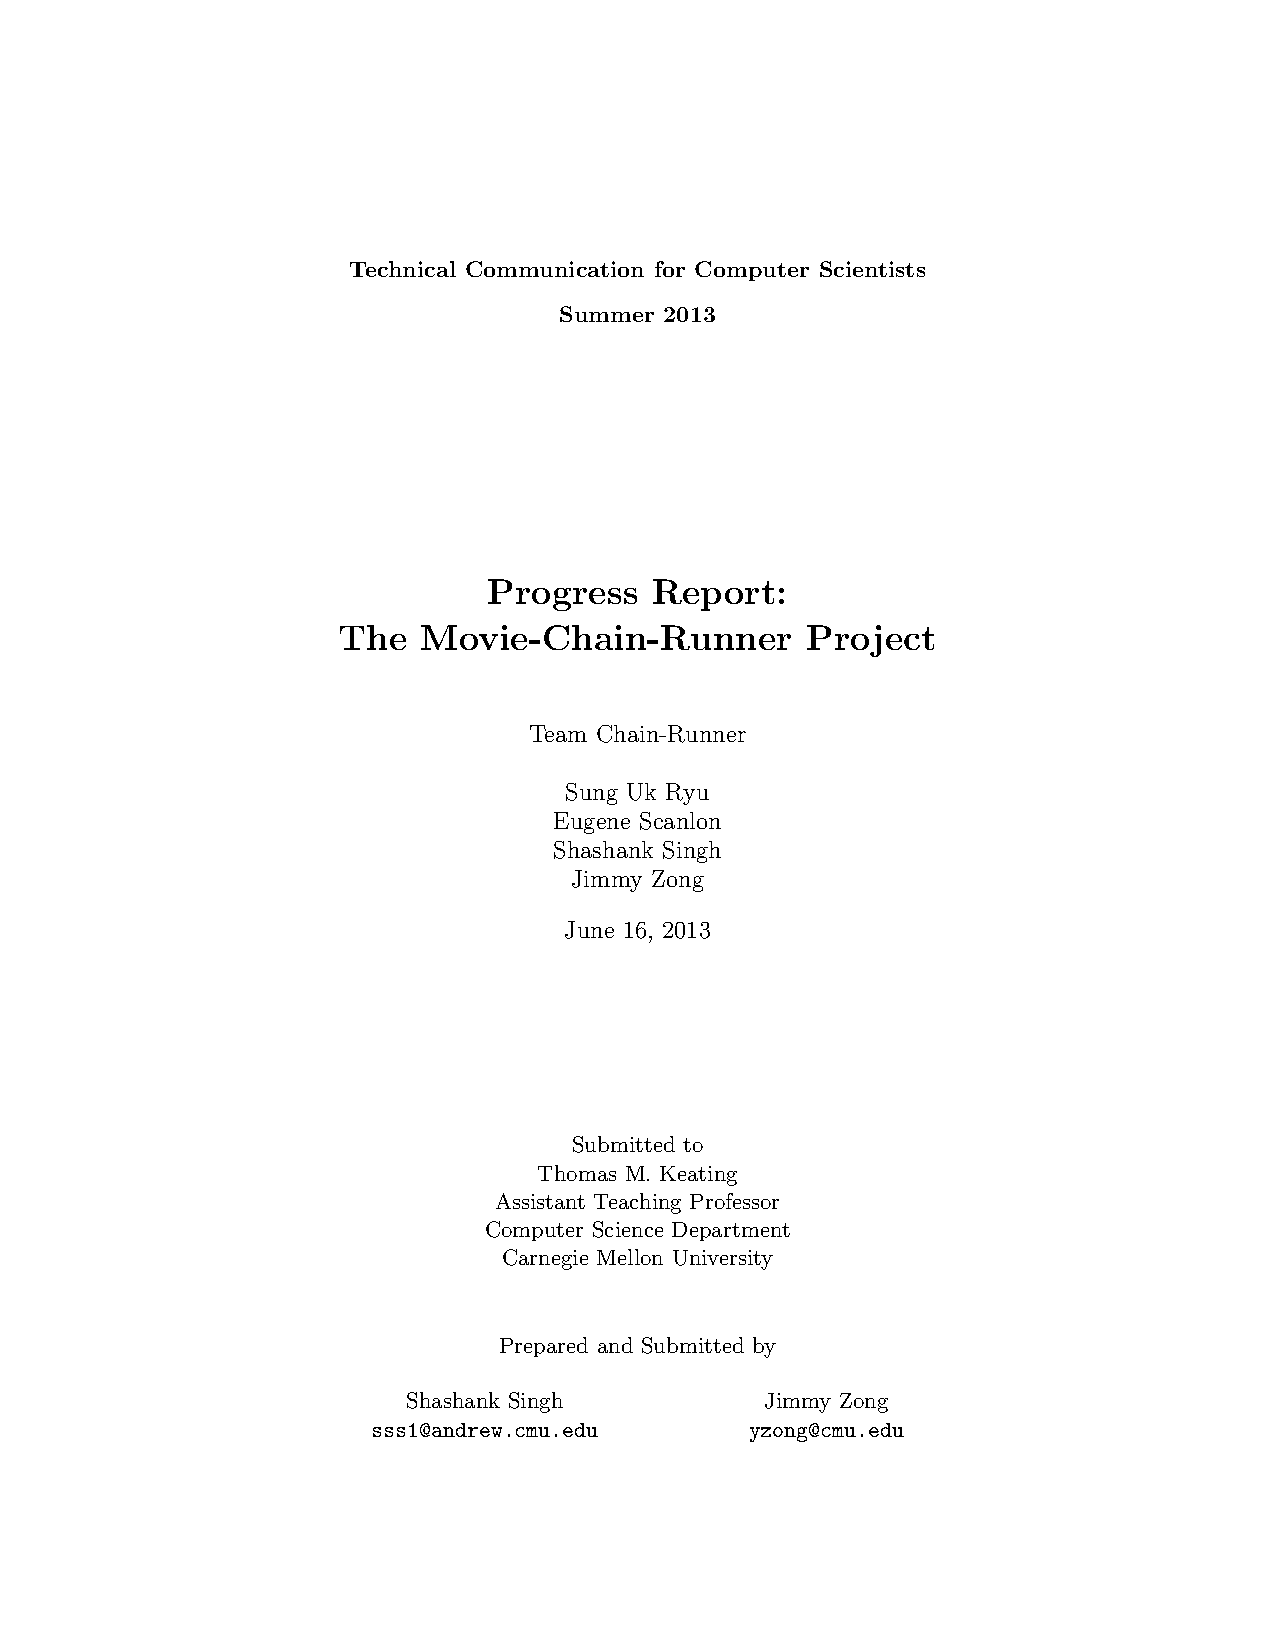
\includepdf{cover/cover.pdf}

\pagenumbering{roman} % include Roman page-numbering on ToC
\tableofcontents

\newpage
\pagenumbering{arabic} % include Arabic page-numbering starting here
\section{Overview}
This report documents our progress on the Movie-Chain-Runner Problem
(discussed in section 2) as of June 17, 2013, as well as our plans for how to
proceed until the project deadline of June 27, 2013. We also discuss and
justify some changes to the plan presented in our project proposal
(submitted June 4, 2013).

\vspace{-0.2cm}
\section{The Movie-Chain-Runner Problem}
The Movie-Chain-Runner Problem is to find the longest chain of overlapping
titles in a list of movie titles, where two titles are said to overlap if some
suffix of the first movie is identical to some prefix of the second movie. For
example, in the list
\begin{itemize}[noitemsep]
\item Day of the Dead
\item Live and Let Die
\item Dead Poets' Society
\item Die Another Day
\item The Last Samurai
\end{itemize}
the longest chain consists of 4 titles:

\begin{center}
Live and Let Die Another Day of the Dead Poets' Society
\end{center}
By appropriately representing the movie list as a graph, the Movie-Chain-Runner
Problem can be shown to be equivalent to the Longest Path Problem (finding the
longest simple path in a directed graph). The Longest Path Problem is well
known to be NP-Complete, meaning that no efficient algorithm exists to find
longest paths in large graphs, including our movie title graph. A review of the
literature reveals that good approximate longest paths also cannot be found
efficiently in large graphs. Thus, our project is to study the movie title
graph and innovate ways to find long paths in the graph.

\vspace{-0.2cm}
\section{Progress}
We discuss our progress in three sections: General Progress, Status, and
Projections.

\vspace{-0.2cm}
\subsection{General Progress}
Our first step was to reconstruct the list of movie titles as a directed graph,
reducing the problem to the well-known Longest Path Problem.
We proceeded to implement a greedy brute force algorithm that simply followed
as many paths as possible. This quickly constructed a path of 243 titles and
then ceased to make appreciable progress.

The majority of our efforts since have been toward augmenting this brute force
algorithm. We have run the algorithm ``backwards'' to extend the beginning of
the chain. We have also attempted running the algorithm in parallel over
several cluster computers, boosting our processing power and thus increasing
the number of possible paths we can check. We are currently running the brute
force algorithm on subsections of the current longest chain, in an attempt to
lengthen the middle of the chain.

We also attempted a theoretically-inspired algorithm which computed acyclic
subgraphs of our graph and then ran a polynomial time Longest Path algorithm
known for directed acyclic graphs. However, the number of cycles proved too
large to generate the subgraphs in a reasonable amount of time, and so we
abandoned this effort.

\vspace{-0.2cm}
\subsection{Status}
Our current longest chain (included in Appendix A) consists of 278 titles,
7 titles short of our June 17 goal of 285 titles. Since extending the movie chain has
proven more difficult than we anticipated, we have decided to scale back our
final goal from 300 titles to 285 titles. Since 285 titles is the necessary
criterion for receiving an A on the project, the benefits of 300 titles are
primarily cosmetic, and so we consider this change acceptable.

Figure \ref{fig:gantto} below shows the original Gantt chart presented in
our project proposal. Figure \ref{fig:ganttn} below shows our revised Gantt
chart, as of June 17. The only changes are that the 300 title goal originally
set for June 25 has been eliminated and the 285 title goal originally set for
June 17 has been extended to June 25.
\begin{figure}[h]
\begin{center}
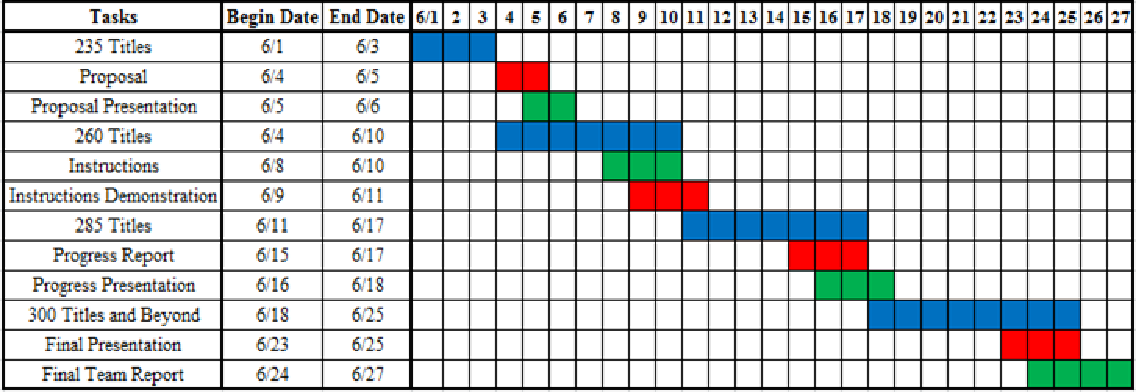
\includegraphics[width=\textwidth]{gantto}
\end{center}
\vspace{-0.7cm}
\caption{Our original Gantt chart.}
\label{fig:gantto}
\end{figure}
\begin{figure}[h]
\begin{center}
\includegraphics[width=\textwidth]{ganttn}
\end{center}
\vspace{-0.7cm}
\caption{Our revised Gantt chart.}
\label{fig:ganttn}
\includegraphics[width=0.2\textwidth]{key}
\end{figure}

\newpage
\subsection{Projections}
We expect that we will accomplish our revised 285 title goal for June 25 and
propose 2 simple approaches to this goal.
Firstly, although we have devoted much computational power toward extending the
longest chain at either end, we have not considered a potentially large number
of alternative paths between nodes in the chain. Thus, we will attempt to
compute, for adjacent or nearby nodes, alternative (longer) chains connecting
the same nodes. Secondly, we are considering ways to ``trim'' the graph by
removing nodes unlikely to be in the longest chain, thus reducing the number of
possible paths that must be considered.

If simple methods prove insufficient, we may also implement a color-coding
algorithm proposed by Alon et al.\hspace{-0.2cm}
\footnote{Noga Alon , Raphael Yuster , Uri Zwick, Color-coding, Journal of the
ACM (JACM), v.42 n.4, p.844-856, July 1995. (accessed June 16, 2013 at
\texttt{http://dl.acm.org/citation.cfm?id=210337}).}
or the genetic algorithms studied by Portugal et al.,\hspace{-0.2cm}
\footnote{
D. Portugal, C. H. Antunes, R. Rocha, ``A Study of Genetic Algorithms for
Approximating the Longest Path in Generic Graphs,'' Proc. of the IEEE SMC, pp.
2539-2544, 2010. (accessed June 16, 2013 at
\texttt{http://ieeexplore.ieee.org/xpl/articleDetails.jsp?arnumber=5641920\&
navigation=1}).}
although, due to the implementation complexity of these algorithms, we hope
this will be unnecessary.

\section{Recomendations}
Our only recomendation is the change of the final project goal from 300 titles
to 285 titles, as discussed in the Progress section above.

\section{Discussion}
Our final deliverable will now be a chain of at least 285 movie titles rather
than a chain of at least 300 movie titles. If, however, we achieve our 285
title goal before our deadline of June 25, we may spend the remaining time
attempting to extend the chain further.

\newpage
\begin{appendices}
\section{Our Longest Movie Chain}
Here, we include our current longest movie chain, with 278 titles and 885
words:
{\footnotesize
\begin{multicols}{2}
\begin{verbatim}
THE RESCUERS
THE RESCUERS DOWN UNDER
UNDER CAPRICORN
CAPRICORN ONE
ONE NIGHT STAND
STAND IN
IN OLD CALIFORNIA
CALIFORNIA SPLIT
SPLIT SECOND
SECOND BEST
BEST OF THE BEST
THE BEST OF EVERYTHING
EVERYTHING RELATIVE
RELATIVE FEAR
FEAR STRIKES OUT
OUT OF THE PAST
PAST MIDNIGHT
MIDNIGHT RUN
RUN SILENT RUN DEEP
DEEP BLUE
BLUE CAR
CAR 54 WHERE ARE YOU
YOU CANT TAKE IT WITH YOU
YOU LIGHT UP MY LIFE
MY LIFE WITHOUT ME
ME MYSELF I
I SPY
SPY HARD
HARD TIMES
TIMES SQUARE
SQUARE DANCE
DANCE WITH A STRANGER
STRANGER IN THE HOUSE
HOUSE OF DRACULA
DRACULA DEAD AND LOVING IT
IT TAKES TWO
24 7 TWENTY FOUR SEVEN
SEVEN YEARS IN TIBET
TIBET CRY OF THE SNOW LION
LION OF THE DESERT
DESERT BLUE
BLUE STEEL
STEEL DAWN
DAWN OF THE DEAD
DEAD BANG
BANG BANG YOURE DEAD
DEAD END
END OF DAYS
DAYS OF HEAVEN
HEAVEN CAN WAIT
WAIT UNTIL DARK
DARK CITY
CITY BY THE SEA
SEA OF LOVE
LOVE AND DEATH
DEATH BECOMES HER
HER MAJESTY MRS BROWN
BROWN SUGAR
SUGAR AND SPICE
SPICE WORLD
WORLD TRADE CENTER
CENTER STAGE
STAGE FRIGHT
FRIGHT NIGHT
NIGHT AND THE CITY
CITY OF JOY
JOY RIDE
RIDE THE HIGH COUNTRY
COUNTRY LIFE
LIFE IS BEAUTIFUL
BEAUTIFUL GIRLS
GIRLS GIRLS GIRLS
GIRLS JUST WANT TO HAVE FUN
FUN AND FANCY FREE
FREE WILLY
FREE WILLY 2 THE ADVENTURE HOME
HOME ALONE
ALONE IN THE DARK
THE DARK HALF
HALF LIGHT
LIGHT OF DAY
DAY FOR NIGHT
NIGHT OF THE LIVING DEAD
DEAD HEAT
HEAT AND DUST
DUST TO GLORY
GLORY ROAD
ROAD GAMES
GAMES PEOPLE PLAY NEW YORK
NEW YORK NEW YORK
NEW YORK COP
COP LAND
LAND OF THE DEAD
DEAD MAN
DEAD MAN ON CAMPUS
CAMPUS MAN
MAN OF THE HOUSE
HOUSE OF FRANKENSTEIN
FRANKENSTEIN AND THE MONSTER FROM HELL
HELL NIGHT
NIGHT FALLS ON MANHATTAN
MANHATTAN MURDER MYSTERY
MYSTERY ALASKA
ALASKA SPIRIT OF THE WILD
THE WILD ANGELS
ANGELS WITH DIRTY FACES
FACES OF DEATH
DEATH SHIP
SHIP OF FOOLS
FOOLS RUSH IN
IN COLD BLOOD
BLOOD BEACH
BEACH PARTY
PARTY GIRL
GIRL IN THE CADILLAC
CADILLAC MAN
MAN ON FIRE
FIRE IN THE SKY
SKY HIGH
HIGH CRIMES
CRIMES OF PASSION
PASSION IN THE DESERT
DESERT HEARTS
HEARTS OF DARKNESS A FILMMAKERS APOCALYPSE
APOCALYPSE NOW
NOW YOU SEE HIM NOW YOU DONT
DONT BOTHER TO KNOCK
KNOCK OFF
OFF THE BLACK
BLACK AND WHITE
WHITE LIGHTNING
LIGHTNING IN A BOTTLE
BOTTLE ROCKET
ROCKET MAN
MAN TROUBLE
TROUBLE EVERY DAY
DAY OF THE DEAD
DEAD OF NIGHT
NIGHT MOTHER
MOTHER JUGS AND SPEED
SPEED 2 CRUISE CONTROL
CONTROL ROOM
ROOM AT THE TOP
TOP GUN
GUN CRAZY
CRAZY AS HELL
HELL UP IN HARLEM
HARLEM RIVER DRIVE
DRIVE ME CRAZY
CRAZY PEOPLE
PEOPLE I KNOW
I KNOW WHAT YOU DID LAST SUMMER
SUMMER CATCH
CATCH A FIRE
FIRE ON THE MOUNTAIN
THE MOUNTAIN MEN
MEN CRY BULLETS
BULLETS OVER BROADWAY
BROADWAY DANNY ROSE
ROSE RED
RED EYE
EYE FOR AN EYE
AN EYE FOR AN EYE
EYE OF GOD
GOD IS GREAT IM NOT
NOT OF THIS EARTH
EARTH GIRLS ARE EASY
EASY MONEY
MONEY FOR NOTHING
NOTHING BUT TROUBLE
TROUBLE IN PARADISE
PARADISE ROAD
ROAD HOUSE
HOUSE PARTY
PARTY MONSTER
MONSTER IN A BOX
BOX OF MOON LIGHT
LIGHT IT UP
UP CLOSE AND PERSONAL
PERSONAL BEST
BEST MEN
MEN WITH GUNS
GUNS OF THE MAGNIFICENT SEVEN
THE MAGNIFICENT SEVEN RIDE
RIDE WITH THE DEVIL
THE DEVIL RIDES OUT
OUT COLD
COLD FEVER
FEVER PITCH
PITCH BLACK
BLACK HAWK DOWN
DOWN WITH LOVE
LOVE LIFE
LIFE OR SOMETHING LIKE IT
IT HAPPENED AT THE WORLDS FAIR
FAIR GAME
GAME OF DEATH
DEATH WISH V THE FACE OF DEATH
DEATH WISH
WISH UPON A STAR
A STAR IS BORN
BORN AMERICAN
AMERICAN HISTORY X
X THE MAN WITH THE X RAY EYES
EYES OF AN ANGEL
ANGEL BABY
BABY SECRET OF THE LOST LEGEND
LEGEND OF THE LOST
THE LOST BOYS
BOYS AND GIRLS
GIRLS WILL BE GIRLS
GIRLS OF SUMMER
SUMMER LOVERS
LOVERS AND OTHER STRANGERS
STRANGERS WHEN WE MEET
MEET JOE BLACK
BLACK LIKE ME
ME WITHOUT YOU
YOU ONLY LIVE ONCE
ONCE AROUND
AROUND THE BEND
BEND OF THE RIVER
THE RIVER WILD
WILD THINGS
THINGS TO COME
COME AND GET IT
IT HAPPENED ONE NIGHT
ONE NIGHT WITH THE KING
THE KING AND I
I WANT TO LIVE
LIVE AND LET DIE
DIE MOMMIE DIE
DIE MONSTER DIE
DIE HARD
HARD EIGHT
EIGHT AND A HALF WOMEN
WOMEN IN LOVE
IN LOVE AND WAR
WAR OF THE WORLDS
THE WORLDS FASTEST INDIAN
INDIAN SUMMER
SUMMER SCHOOL
SCHOOL OF ROCK
ROCK STAR
STAR TREK THE MOTION PICTURE
PICTURE BRIDE
BRIDE OF THE WIND
THE WIND AND THE LION
THE LION KING
KING OF THE JUNGLE
JUNGLE 2 JUNGLE
JUNGLE BOOK
BOOK OF LOVE
LOVE WALKED IN
IN GODS HANDS
HANDS ON A HARD BODY
BODY DOUBLE
DOUBLE TEAM
TEAM AMERICA WORLD POLICE
POLICE ACADEMY
POLICE ACADEMY 3 BACK IN TRAINING
TRAINING DAY
DAY OF THE WOMAN
THE WOMAN IN RED
RED RIVER
RIVER OF NO RETURN
RETURN TO HORROR HIGH
HIGH SCHOOL HIGH
HIGH SPIRITS
SPIRITS OF THE DEAD
DEAD MAN WALKING
WALKING AND TALKING
TALKING ABOUT SEX
SEX AND THE OTHER MAN
MAN OF THE YEAR
YEAR OF THE DRAGON
DRAGON SEED
SEED OF CHUCKY
\end{verbatim}
\end{multicols}
}
\end{appendices}
\end{document}
